\chapter{Technical Detail}

\section{Collaborative Downlaod}
ColStream assigns one of two roles to its users, initiators and collaborators. A user streaming a video is an initiator. Users offering their bandwidth to others are collaborators. The initiator creates a group of potential collaborators and assigns them chunks of the video stream data to download, based on their capabilities and price demands. The figures \ref{grpfrm1} and \ref{grpfrm2} illustrate the process of group formation, respectively the actual download of video information by role. 

\section{Group formation}

\begin{figure}[hbtp]
\centering
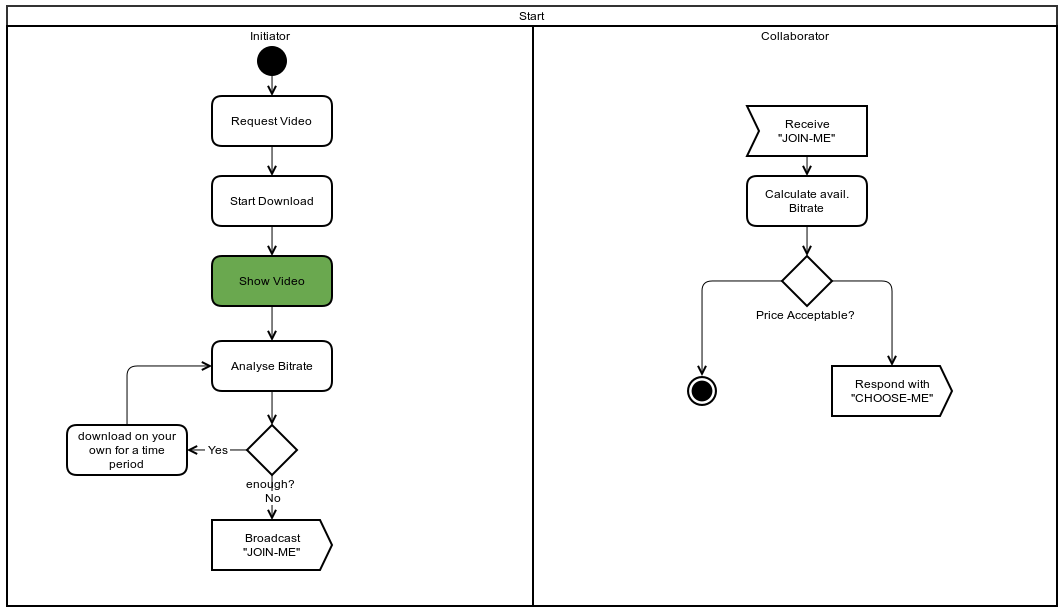
\includegraphics[scale=.6]{figures/Workflow_1.png}
\caption{Group formation}
\label{grpfrm1}
\end{figure}
% \label{groupformation1}


In the left half of figure \ref{grpfrm1} we see the behaviour of an initiator when he begins to stream a video. He starts by downloading and showing the video on its own. The initiator then analyses the bitrate at which he receives the video information. If this bitrate is enough to provide the user with an acceptable video quality, the initiator keeps streaming the video on its own and periodically rechecks the bitrate. Should at some point the bitrate be no longer acceptable, the initiator tries to form a group with collaborators. To find candidates for a group, the initiator broadcasts a "JOIN-ME" message. This message contains information on the amount of required bandwidth as well as how much the initiator is willing to pay for this bandwith. Potential collaborators in range of the initiator will receive the "JOIN-ME" request and process it as shown in the right half of figure \ref{grpfrm1}. Each collaborator first calculates the bitrate he could offer to the initiator based on the signal strength of the 4G/LTE network. He then compares the price offered by the initiator to his own current demand. Limited resources like battery capacity can drive the price up. Should the offered price be acceptable to the collaborator, he responds with a "CHOOSE-ME" message to indicate his consent to join the group.

\subsection{Bitrate estimation}
The collaborators estimate the bitrate they can offer to the initiator based on their signal strentgh. To be able to do this in a realistic way, collaborators periodically measure their signal and the corresponding bitrate. To compensate for fluctuations, historic information is factored into these measurements. The specific equations are 
\begin{itemize}
\item $signal=\alpha * signal_{new}+(1-\alpha)* signal_{old}$
\item $tp=\alpha * tp_{new}+(1-\alpha)* tp_{old}$
\end{itemize} with tp being throughput and \alpha an unspecified factor.

\section{Collaborative download}
The process of collaborative streaming within the group created in the previous section is shown in figure \ref{grpfrm2}.
Based on the "CHOOSE-ME" messages received by the initiator, a pool of possible participants in the streaming is created. The initiator then periodicly selects the best suited candidate to download a chunk of the video stream and assignes him this task by sending a request to do so. The size of the chunks is dynamically calculated to fit the throughput the candidates provide, using this equation:  \begin{itemize}
%{\frac{{MAX_CHUNK_SIZE * tp_{i}}{tp_{max}}}}equation  \begin{itemize}
%{\frac{{MAX_CHUNK_SIZE * tp_{i}}{tp_{max}}}}
\item $Chunk Size_{i}=\frac{MAX CHUNK SIZE * tp_{i}}{tp_{max}}$
\end{itemize}
Candidates are selected based on their price demand and offered bitrate. On receiving a download request, a collaborator downloads the assigned chunk of the stream and forwards it as a message to the initiator. When the initiator receives this message, he integrates the data into the video stream and displays it to the user.
The number of collaborators available to an initiator is expected to be changing over time. The collaborators send regular "I-AM-ALIVE" messages to the initiator to indicate that they are still available. They initiator will tolerate up to three missed messages in a row before dismissing the collaborator as not longer available.


%Workflow for the structure of collaboration
\begin{figure}[hbtp]
\centering
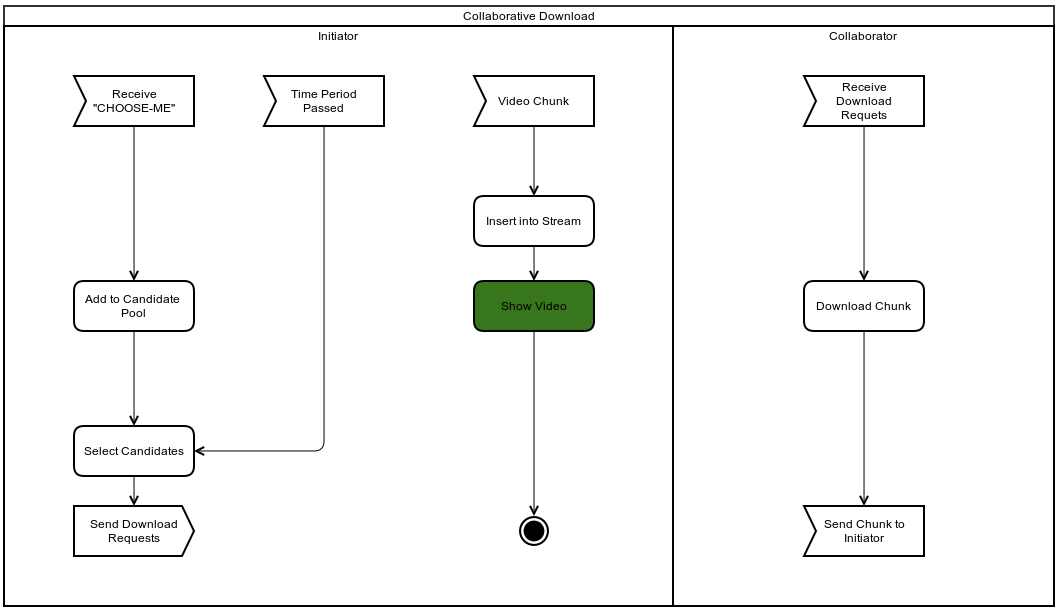
\includegraphics[scale=.6]{figures/Workflow_2.png}
\caption{Collaborative Download}
\label{grpfrm2}
\end{figure}


% \section{Working Algorighm}
\subsection{Problem handling}
The work is distributed between collaborators through assignment of chunks of the video. However once these chunks are assigned, a number of problems might appear that will make it impossible for the collaborator to complete the download on time. For example the user might experience interference which will drop his network throughput below the expected value. In this situation ColStream collaborators notify the initiator of the problem and forward the already downloaded information to him, so he has to reassign the remaining part only. Another problem is the loss of Wi-Fi connection to one of the collaborators. The initiator can notice this loss through missing "I-AM-ALIVE" messages or if the collaborator takes longer then expected to provide a chunk. If the collaborator does not respond to additional messages, the initiator will download this collaborators chunk on his own to compensate for the missing data.